\documentclass[a4paper,runningheads]{llncs}

\usepackage[T1]{fontenc}
\usepackage{graphicx}
\usepackage{array}
\usepackage{booktabs}
\usepackage{amsmath}
\usepackage{amssymb}
\usepackage{amsfonts}
\usepackage[hidelinks]{hyperref}

\begin{document}

% The full title uses a colon; LNCS sets the post-colon part as subtitle.
\title{Sem2Act: Diagnosing Retrieval Value Loss from Evidence to Action in Stateful Decision Systems}
\titlerunning{Sem2Act}
\hypersetup{pdftitle={Sem2Act: Diagnosing Retrieval Value Loss from Evidence to Action in Stateful Decision Systems}}

\author{Anonymous Author(s)}
\authorrunning{Anonymous}
\institute{Anonymous Institution}

\maketitle

\begin{abstract}
Retrieval utility is increasingly studied in RAG, but consequential decision systems introduce a different problem: retrieved evidence changes beliefs and actions whose effects persist through future state. We introduce Sem2Act, a frozen paired benchmark that traces evidence through an information consumer, probabilistic belief, fixed decision policy, and stateful environment to measure realized sequential utility.

Across 160 held-out queries and five paired seeds, at $k=3$, all tested
real-retriever arms under naive LLM consumption reduce paired return
relative to NoInfo, while oracle-selected evidence through the same
consumer improves return by up to $+178.9$. Sem2Act then diagnoses where
that value is lost: pre-specified leave-one-out contrasts reveal
consumer-conditioned, including opposite-signed, removal effects; selected
directions and their ordering replicate from development to held-out test.
Provenance-aware consumption reduces interpretation gaps from $140.5$
to $36.4$ (8B) and from $144.8$ to $52.9$ (14B), but real-rerank arms
remain non-positive. Finally, a pre-specified and frozen
label-free predictor of passage value fails to transfer to held-out data,
exposing the gap between retrospective measurement and prospective
prediction.

Sem2Act therefore extends utility-centric retrieval evaluation to
fixed-policy stateful decision systems, where retrieved evidence affects
actions and persistent environment state.
\keywords{Retrieval evaluation \and Downstream utility \and Evidence selection
\and Consumer dependence \and Negative results.}
\end{abstract}

\section{Introduction}
\label{sec:intro}

Traditional retrieval metrics evaluate evidence before observing its
downstream use: they score retrieved passages without seeing what any
downstream system does with them. Yet the same retrieved set can be
transformed differently by different consumers, so a relevance gain need
not survive the handoff. That topical relevance can diverge from task
value is textbook~\cite{borlund2003concept}, and RAG studies have
quantified single-step versions: weak relevance-to-utility
proxy~\cite{salemi2024erag}; model-specific
grounding utility~\cite{grogu2026}; stronger retrievers retrieving harder
distractors~\cite{cuconasu2024power,yoran2024making}. We study a less
explored continuation: following retrieved evidence through a fixed
consumer and decision policy into persistent environment state and
realised return.

We study that transfer in a controlled testbed: an operator triages a
stream of supply-network reports, most about other sites, some stale, a
few demanding a changed order. The inventory simulator is the laboratory
instrument --- fixed, paired, fully observable --- and the research
contribution is the evaluation design around it.

Our central retrieval question: \emph{when does
retrieval relevance transfer into downstream utility, and where is that
value lost when it does not?} Sem2Act extends, not replaces, standard
relevance evaluation: its first layer scores BM25, dense, hybrid and
reranked systems by nDCG@10, and each later layer follows the evidence
one step further --- consumer, belief, action, realised return
(Figure~\ref{fig:sem2act}).

\begin{equation}
\label{eq:path}
q,\,\mathcal{D} \;\longrightarrow\; R_k(q,\mathcal{D}) \;\longrightarrow\;
b(z\mid \cdot) \;\longrightarrow\; \pi(a_t\mid s_t,b) \;\longrightarrow\;
s_{t+1} \;\longrightarrow\; U.
\end{equation}

A retrieval system $R_k$ selects $k$ documents from $\mathcal{D}$; a fixed
consumer maps them to a belief $b$; a fixed controller maps state and
belief to an action; a simulator returns realised utility $U$. Shared
seeds enable paired comparisons of evidence-selection interventions
while downstream components and stochastic worlds are held fixed;
varying only the consumer yields a matched comparison of consumption
effects.

\begin{figure}[!tb]
\centering
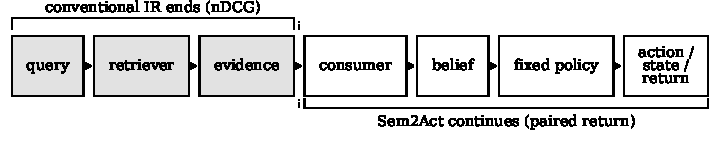
\includegraphics[width=\textwidth]{figures/fig1_sem2act}
\caption{Sem2Act evaluation flow (schematic of Eq.~(1)): the same
evidence is followed through consumption, belief, a fixed policy, and
persistent state to realised return.}
\label{fig:sem2act}
\end{figure}

\paragraph{The result.}
At $k=3$, real retrieval reduces operating return for naive-LLM (C1)
consumers under the frozen pipeline (C1/8B: $-103.5$ BM25 to $-43.6$
rerank; C1/14B effects range from $-93.2$ to $-40.9$; all eight
real-retriever C1 arms
Holm-robust), while oracle evidence through
the same machinery adds up to $+178.9$. A development-tuned no-text
belief reaches $1881.1$ ($+102.1$),
beating every real-retriever arm. The four-gap ladder (rerank arm)
attributes the shortfall to selection ($+79.5$ to $+200.7$), zero veracity
gap ($0.00$), interpretation ($140.5 \to 36.4$), and a dominating control
gap of $+456.8$.

\paragraph{Contributions.}
(i) Sem2Act, a controlled framework for evaluating retrieval utility in
sequential decisions: the same evidence scored first by
conventional relevance (nDCG@10), then by sequential realised return
through a fixed consumer, belief, policy and persistent
environment --- matched budgets, paired randomisation, and an oracle
ladder separating selection, veracity, interpretation and control
(Section~\ref{sec:transfer}--\ref{sec:ladder}).
(ii) The mismatch pattern this instrument reveals, measured per
consumer: passage-removal interventions, a no-text comparator no real
retriever beats, a rule-vs-LLM interaction, and a four-gap
attribution (Sections~\ref{sec:utility}--\ref{sec:ladder}).
(iii) A statistical discipline for this design: paired shared-seed worlds,
crossed bootstrap, Holm over 105 arms, text-cluster honesty
check (Section~\ref{sec:uncertainty}), with every table regenerating from
stored episodes.

\paragraph{Scope.} Synthetic feed and environments; constructed,
non-human-assessed relevance (Section~\ref{sec:limitations}). Claims are
about \emph{evaluation}, scoped to arms, priors and environments where
corrections hold.

\section{Related work}
\label{sec:related}

\paragraph{What we inherit.}
Relevance-vs-value divergence is established (Figure~\ref{fig:timeline}
traces the lineage): task-based relevance
critique~\cite{borlund2003concept}; eRAG's weak
relevance-to-utility proxy~\cite{salemi2024erag}; model-specific
grounding utility~\cite{grogu2026}; distracting passages whose harm grows
with retriever strength~\cite{cuconasu2024power,yoran2024making}.
Distraction reaches even strong models~\cite{shi2023large}, and
component-wise RAG evaluation exists~\cite{saadfalcon2023ares,es2023ragas}.
Retrieval-augmented generation couples retriever and generator, where
higher retrieval accuracy \emph{does} raise end-task
accuracy~\cite{lewis2020rag,karpukhin2020dpr}. The same holds for
utility-trained retrievers~\cite{xu2025scarlet} and LLM-oriented gain
metrics~\cite{trappolini2026redefining}; RRPO directly optimizes reranking
with LLM feedback for downstream generation utility~\cite{wu2026rrpo}.
Prospective RAG work also predicts retrieval utility and answer quality from
query-, document-, and reader-side features~\cite{tian2026predicting}.
Most primarily evaluate
answer-level or retrieval-stage utility; recent agentic work additionally
studies utility across multi-step retrieval
trajectories~\cite{mukhopadhyay2026bridge}. That
prediction quality differs from decision quality is established across
task-based learning~\cite{donti2017task,elmachtoub2022smart,mandi2022rank};
value-aware dynamics~\cite{farahmand2017value,lambert2020objective};
and decision calibration~\cite{zhao2021decision}. Value of
information, search economics, and proper
scoring provide the footing~\cite{howard1966information,azzopardi2011economics,guo2017calibration,degroot1983comparison,niculescu2005predicting}. \emph{None of these claims is ours:} each could have
explained our results; the controls below test those explanations. Closest are decision-focused inventory learning (we
freeze the trained loop and vary only the
supplied text) and the SPO
loss~\cite{elmachtoub2022smart}, which our $\Delta J$ applies to retrieved
evidence. Operational LLM systems have also been studied in supply-chain
and inventory settings~\cite{li2023optiguide,yoshizato2026agents}; those
works primarily optimize or evaluate the acting agent, whereas Sem2Act
holds the downstream policy and simulator fixed to diagnose where
retrieval value is lost (see
Table~\ref{tab:contrib} for the closest-work comparison).

\begin{figure}[tb]
\centering
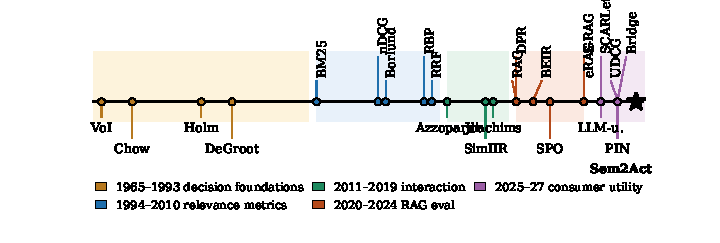
\includegraphics[width=\textwidth]{figures/fig_timeline}
\caption{Retrieval-evaluation lineage (selected milestones; years are
publication years of cited works; recent years are expanded horizontally
for readability). Decision foundations, relevance
metrics, interaction economics, RAG evaluation, and consumer-conditioned
utility converge on Sem2Act (star), which adds sequential realised return
under a fixed policy and persistent state.}
\label{fig:timeline}
\end{figure}



\subsection{What remains novel}
To our knowledge, prior retrieval-utility evaluations do not combine
retrieved evidence, a separately varied consumer, a fixed sequential
controller, paired persistent-state simulation, matched budgets, and an
oracle diagnostic ladder in one evaluation
(Table~\ref{tab:contrib} differentiates each closest contribution).
SIVR is a skill-score-style normalization for diagnostic bookkeeping,
not a methodological contribution. Simulation as evaluation has
IIR precedent~\cite{maxwell2016simiir}; where that work simulates the
searcher, Sem2Act simulates the consumer-to-action path.

\begin{table}[t]
\centering
\caption{Closest contributions vs Sem2Act (factual summary; the final row is
this work). The right column states narrowly
what Sem2Act adds in each case.}
\label{tab:contrib}
{\footnotesize
\begin{tabular}{>{\raggedright\arraybackslash}p{2.5cm}
                >{\raggedright\arraybackslash}p{4.0cm}
                >{\raggedright\arraybackslash}p{4.45cm}}
\toprule
Work & Closest contribution & Added by Sem2Act \\
\midrule
SCARLet~\cite{xu2025scarlet} & utility-trained retrieval &
value evaluation without retraining; dev$\to$test replication \\
UDCG~\cite{trappolini2026redefining} & LLM utility metric tied to answer accuracy &
sequential return under persistent state \\
LLM-specific~\cite{zhang2025llmspecific} & reader-specific utility; weak transfer &
fixed boundary and policy/state failure test \\
Bridge~\cite{mukhopadhyay2026bridge} & static versus causal utility gap &
fixed-policy interventions and oracle ladder \\
PIN~\cite{zhou2026preference} & cross-reader transfer failure &
per-consumer effects under the same boundary \\
Sem2Act & consumer-conditioned value in a frozen benchmark & --- \\
\bottomrule
\end{tabular}
}
\end{table}

\section{Framework: Sem2Act}
\label{sec:framework}

We name the instrument \emph{Sem2Act}: diagnosing retrieval value loss
from evidence to action in a stateful decision system, across the five
stages of~\eqref{eq:path}. Sem2Act is a frozen evaluation discipline,
not a retrieval model: it varies retrievers and consumers separately
while holding policy and simulator fixed, so retrieval, consumption,
and action-sensitivity effects are measured, not collapsed.



\subsection{Objects and estimand}

Let $z$ be a latent operational regime, $\mathcal{D}$ a candidate pool of
reports and $q$ a fixed query expressing a standing information need. A
retrieval system returns an ordered list; its top $k$ documents are the
evidence. A fixed consumer maps that evidence to a belief $b(z)$, and a fixed
controller maps state and belief to an action.

Write $G_i(m)$ for the \emph{realised} return of episode $i$ under information
source $m$, $G_i(m)=\sum_{t=0}^{T-1} r(s^{(i)}_t,a^{(i)}_t,z^{(i)})$,
undiscounted over the fixed $T=40$ horizon. Its expectation is estimated by
the weighted benchmark return
\begin{equation}
\label{eq:jw}
J_w(m) \;=\; \sum_{r} w_r \,
\operatorname*{mean}_{f \in \mathcal{F}_r} \;
\operatorname*{mean}_{v \in \mathcal{V}_{r,f}} \;
\operatorname*{mean}_{i \in \mathcal{S}} \; G_i(m; r, f, v),
\end{equation}
averaging seeds within a query $v$, queries within a family $f$, families
within a regime $r$, and combining regimes with declared weights $w_r$. The
\emph{balanced} estimand uses uniform $w_r$ and is primary; an
\emph{empirical} estimand matching the test bank mix is reported alongside
every headline.

Effects are paired differences $\Delta J$ against a declared
reference (no-retrieval control; uninformed prior for consumers) on the
160 held-out test queries. Gaps
are signed differences of balanced $J$ across the ladder rungs
(Section~\ref{sec:ladder}); a development-tuned constant no-text belief
(Section~\ref{sec:tuned}) is the stronger comparator. The
diagnostic $\mathrm{SIVR}$ against both
reference beliefs carries an explicit guard; it is bookkeeping. Every
effect we report is a \emph{realized} information effect of forcing a
fixed, imperfect pipeline to ingest evidence, and can be negative ---
unlike classical value of information, which is nonnegative when the
decision maker can optimally use or ignore additional
information~\cite{howard1966information}. \textsc{PerfectBelief} is
not an upper bound on achievable return, because
\textsc{HindsightOracle} also improves the controller; we report raw
paired effects first.

\subsection{Uncertainty}
\label{sec:uncertainty}

Queries are the primary unit; five paired seeds ($60000$--$60004$) quantify
environmental uncertainty, shared
across every treatment: every query is evaluated on the same seeds, so we
resample one \emph{shared} seed sample per regime plus queries with
replacement
(crossed bootstrap, $B=5{,}000$; $p$-values bounded below by $1/(B+1)$).
Paired randomisation testing
follows IR practice~\cite{smucker2007comparison}, as counterfactual
evaluation does from biased feedback~\cite{joachims2017unbiased};
family-wise control follows classifier-comparison
practice~\cite{demsar2006statistical}. Semantic statistics use paired
query bootstrap ($B=10{,}000$). Multiplicity is controlled by Holm
adjustment~\cite{holm1979simple} over the 105-arm utility family and ten preregistered
headline semantic cells; all other contrasts are reported as estimates
with CIs. Honesty provisions: 200 IDs share 64
texts (63 test) --- a text-cluster bootstrap (median $1.08\times$ wider;
practice follows~\cite{cameron2008bootstrap}) backs every starred claim
(effective $N\approx137$); inference is to new queries/seeds \emph{within
this bank}; regime-conditional statements are exploratory
($n=5$ seeds).

\section{Retrieval to semantic transfer}
\label{sec:transfer}

The first experimental layer is conventional retrieval evaluation, on the
same queries and episodes the later layers reuse (200 queries over
a 64-node feed, 40 dev / 160 test incl. 16 held-out entities;
test seal held until frozen analysis).
Systems: random, BM25~\cite{robertson1994okapi}, instructed
Qwen3-Embedding-0.6B dense~\cite{zhang2025qwen3embedding}, RRF hybrid
($k=120$)~\cite{cormack2009reciprocal}, reranker over
hybrid top-30, oracle ceilings, seven
prespecified interventions; scored with nDCG~\cite{jarvelin2002cumulated}
in its user-model lineage~\cite{moffat2008rbp}. Consumers C0/C1/C3: C0 (rule-based,
model-free), C1 (naive LLM use), C3 (per-document extraction,
$\tau=0.5$; abstentions carry the prior, score $0$ accuracy
--- a reject option~\cite{chow1970optimum}). Two pinned open-weight
models (8B/14B); 11{,}018 content-addressed cache files, zero assembly writes.

\begin{table}[t]
\centering
\caption{Retrieval quality on the 160 test queries (trec\_eval; 95\% query-bootstrap CIs: BM25 $[0.095,0.135]$, dense $[0.153,0.198]$, hybrid $[0.157,0.207]$, rerank $[0.156,0.210]$ --- point-ordered with overlapping intervals). R@k is recall at $k$. The frozen ranker is RRF over BM25 and instructed dense embeddings ($k=120$) with reranker depth 30, selected on dev only.}
\label{tab:retrieval}
\begin{tabular}{lcccc}
\toprule
System & nDCG@10 & R@10 & R@20 & MRR \\
\midrule
BM25 & 0.1150 & 0.1365 & 0.2604 & 0.2102 \\
Dense & 0.1754 & 0.2062 & 0.3771 & 0.2656 \\
Hybrid RRF & 0.1817 & 0.2167 & 0.4094 & 0.2857 \\
Reranked & 0.1829 & 0.1938 & 0.3708 & 0.2812 \\
\bottomrule
\end{tabular}
\end{table}


Table~\ref{tab:retrieval} and Figure~\ref{fig:irquality} show the frozen
ranker is point-ordered
(BM25 $0.115$ to reranked $0.183$; dense/hybrid/rerank intervals overlap),
though rerank's edge over hybrid shrinks out of sample ($+0.024$ dev $\to$
$+0.001$ test). Relevance differences are modest by construction: qrels fix
only this conventional layer, while sequential utility is measured
independently downstream.

\begin{figure}[!tb]
\centering
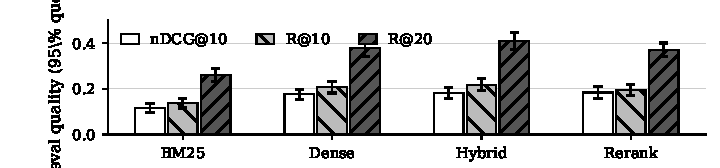
\includegraphics[width=\textwidth]{figures/fig_ir_quality}
\caption{Conventional retrieval quality on the 160 test queries
(nDCG@10, R@10, R@20, each with 95\% query-bootstrap CIs, $B=10{,}000$).
Dense and hybrid/reranked improve nDCG over BM25 ($0.115\to0.183$);
the reranker trades recall (R@10 $0.217\to0.194$).}
\label{fig:irquality}
\end{figure}

\begin{table}[t]
\centering
\caption{Semantic quality on test queries at $k=3$ (160 queries). Abstention rates: C3/random 0.56--0.94, else $\le 0.03$. A C3 abstention scores $0$ accuracy while retaining the prior for Brier. Per-cell CIs (median half-width $0.07$) are in the anonymous supplementary artifact.}
\label{tab:semantic}
(a) Regime accuracy\\[2pt]
{\small\setlength{\tabcolsep}{4pt}
\begin{tabular}{lccccc}
\toprule
System & C0 & C1/8B & C1/14B & C3/8B & C3/14B \\
\midrule
BM25 & 0.406 & 0.275 & 0.338 & 0.344 & 0.338 \\
Dense & 0.412 & 0.287 & 0.281 & 0.388 & 0.331 \\
Hybrid & 0.425 & 0.362 & 0.350 & 0.375 & 0.350 \\
Rerank & 0.400 & 0.406 & 0.412 & 0.444 & 0.444 \\
Random & 0.350 & 0.237 & 0.225 & 0.081 & 0.006 \\
Oracle & 0.594 & 0.700 & 0.719 & 0.963 & 0.969 \\
\bottomrule
\end{tabular}
}
\\[6pt](b) Brier score\\[2pt]
{\small\setlength{\tabcolsep}{4pt}
\begin{tabular}{lccccc}
\toprule
System & C0 & C1/8B & C1/14B & C3/8B & C3/14B \\
\midrule
BM25 & 0.254 & 0.356 & 0.314 & 0.271 & 0.288 \\
Dense & 0.233 & 0.329 & 0.319 & 0.260 & 0.282 \\
Hybrid & 0.260 & 0.315 & 0.291 & 0.263 & 0.273 \\
Rerank & 0.297 & 0.258 & 0.257 & 0.269 & 0.262 \\
Random & 0.286 & 0.336 & 0.327 & 0.252 & 0.226 \\
Oracle & 0.157 & 0.121 & 0.127 & 0.028 & 0.035 \\
\bottomrule
\end{tabular}
}
\end{table}


Semantic accuracy (Table~\ref{tab:semantic}, Figure~\ref{fig:semheat})
sits at $0.275$--$0.450$ outside
abstention-collapse cells --- barely above model-free C0 on identical evidence
and far below oracle evidence (C3: $0.96$--$0.97$). Scale shows no
systematic advantage (34 of 42 8B-vs-14B Q6 cells null,
max $|\Delta|$ $0.144$); only C1/8B preserves the
BM25 $<$ Dense $<$ Hybrid $<$ Rerank order exactly, while the other LLM
columns contain reversals and absolute accuracy stays low.

\begin{figure}[!tb]
\centering
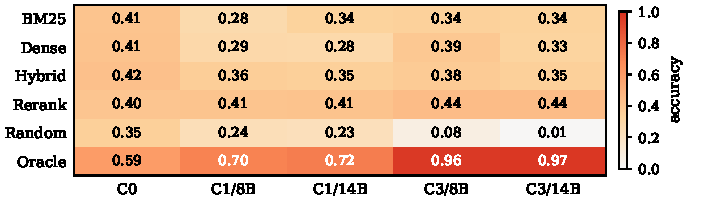
\includegraphics[width=\textwidth]{figures/fig_semantic_heatmap}
\caption{Semantic accuracy at $k=3$ (160 test queries) by retriever and
consumer (C0 rule-based, C1 naive LLM, C3 provenance-aware; 8B/14B
models; Oracle = oracle-relevant). C1 underperforms model-free C0 on
identical evidence in 6 of 8 real-retriever cells (all but rerank; 16 of
20 non-oracle LLM cells below C0); oracle evidence
reaches $0.96$+ only under C3; random evidence collapses C3
($0.08$/$0.01$) via abstention.}
\label{fig:semheat}
\end{figure}

\begin{table}[t]
\centering
\caption{Prespecified semantic contrasts at $k=3$ (accuracy; paired 95\% CIs; Holm $p$ over ten cells; Q3 = cross-consumer rerank--BM25 differences, Q5 = C3--C1 at rerank, Q6 = 8B--14B at rerank). $^*$ denotes Holm rejection (Q6/C3 degenerate).}
\label{tab:interaction}
\begin{tabular}{lcc}
\toprule
Contrast & Effect [95\% CI] & Holm $p$ \\
\midrule
Q3: $C0-C1$ (8B) & $-0.138$ $[-0.225,-0.056]$ & $0.0150^*$ \\
Q3: $C0-C3$ (8B) & $-0.106$ $[-0.175,-0.037]$ & $0.0360^*$ \\
Q3: $C1-C3$ (8B) & $+0.031$ $[-0.050,+0.113]$ & $1.0000$ \\
Q3: $C0-C1$ (14B) & $-0.081$ $[-0.150,-0.013]$ & $0.1855$ \\
Q3: $C0-C3$ (14B) & $-0.113$ $[-0.188,-0.037]$ & $0.0297^*$ \\
Q3: $C1-C3$ (14B) & $-0.031$ $[-0.087,+0.025]$ & $1.0000$ \\
Q5: $C3-C1$ (8B) & $+0.037$ $[-0.019,+0.094]$ & $1.0000$ \\
Q5: $C3-C1$ (14B) & $+0.031$ $[-0.019,+0.081]$ & $1.0000$ \\
Q6: $8B-14B$ (C1) & $-0.0063$ $[-0.0312,+0.0187]$ & $1.0000$ \\
Q6: $8B-14B$ (C3) & $+0.0000$ $[+0.0000,+0.0000]$ & $1.0000$ \\
\bottomrule
\end{tabular}
\end{table}


The retriever$\times$consumer interaction (Table~\ref{tab:interaction}) is
carried by rule-vs-LLM contrasts (3/10 Holm-robust); C1-vs-C3
differences retain nulls. All LLM consumers are pinned
Qwen-family models, so the evidence shows dependence on the consumption
mechanism, not broad variability among arbitrary LLM consumers
(concurrent work finds the same boundary~\cite{zhang2025llmspecific,zhou2026preference}).

\section{Sequential utility}
\label{sec:utility}

Replaying frozen beliefs through the frozen controller and simulator
gives Table~\ref{tab:utility} and Figure~\ref{fig:rxc} (headlines use
the 160 test queries).

\begin{table}[t]
\centering
\caption{Paired $\Delta J$ vs no-retrieval control at $k=3$ (160 test queries $\times$ 5 seeds; crossed bootstrap, $B=5{,}000$). $^*$: Holm rejection (105 arms); unstarred cells Holm-n.s. Displayed CIs are unadjusted; stars carry multiplicity control. A harm claim is headlined only if Holm-robust under balanced weights and same-signed under empirical weights. Cluster CIs (median $1.08\times$, max $1.19\times$) agree in direction for every starred cell. Refs: NoInfo $1779.0$, PerfectBelief $1994.4$, Hindsight $2451.2$. NoText\_Tuned $1881.1$ (\S\ref{sec:tuned}).}
\label{tab:utility}
{\small\setlength{\tabcolsep}{1pt}\renewcommand{\arraystretch}{1.0}
\begin{tabular}{@{}>{\raggedright\arraybackslash}p{1.35cm}*{5}{>{\centering\arraybackslash}p{1.85cm}}@{}}
\toprule
System & C0 & \shortstack{C1\\8B} & \shortstack{C1\\14B} & \shortstack{C3\\8B} & \shortstack{C3\\14B} \\
\midrule
BM25 & $-8.5$ & $-103.5^*$ & $-89.7^*$ & $-43.4$ & $-59.8^*$ \\
 & $[-32,+16]$ & $[-137,-71]$ & $[-118,-63]$ & $[-71,-15]$ & $[-82,-37]$ \\
\addlinespace[1pt]
Dense & $-4.6$ & $-91.5^*$ & $-93.2^*$ & $-27.9$ & $-55.2^*$ \\
 & $[-26,+17]$ & $[-122,-61]$ & $[-121,-66]$ & $[-58,+3]$ & $[-79,-31]$ \\
\addlinespace[1pt]
Hybrid & $-9.8$ & $-74.6^*$ & $-73.9^*$ & $-36.6$ & $-54.4^*$ \\
 & $[-35,+15]$ & $[-105,-44]$ & $[-97,-51]$ & $[-64,-10]$ & $[-73,-35]$ \\
\addlinespace[1pt]
Rerank & $-40.2$ & $-43.6^*$ & $-40.9^*$ & $-21.8$ & $-20.7$ \\
 & $[-68,-13]$ & $[-65,-23]$ & $[-62,-20]$ & $[-56,+11]$ & $[-48,+7]$ \\
\addlinespace[1pt]
Random & $-35.0$ & $-90.4^*$ & $-89.9^*$ & $-13.1$ & $+10.9^*$ \\
 & $[-62,-9]$ & $[-110,-71]$ & $[-104,-75]$ & $[-26,-2]$ & $[+7,+14]$ \\
\addlinespace[1pt]
Oracle & $+39.3$ & $+74.9^*$ & $+70.6^*$ & $+178.9^*$ & $+162.5^*$ \\
 & $[+9,+69]$ & $[+38,+111]$ & $[+32,+108]$ & $[+135,+221]$ & $[+125,+200]$ \\
\bottomrule
\end{tabular}
}
\end{table}


\begin{figure}[!tb]
\centering
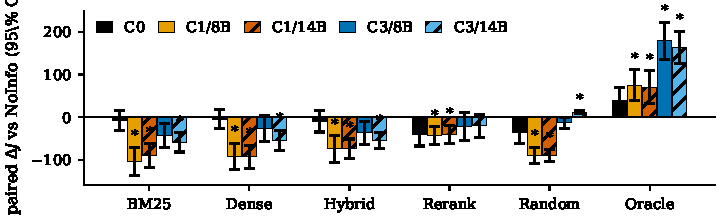
\includegraphics[width=\textwidth]{figures/fig2_rxc_full}
\caption{Full retriever$\times$consumer matrix (paired $\Delta J$ vs
NoInfo, $k=3$, 160 test queries $\times$ 5 seeds, crossed 95\% CIs,
$*$ Holm-robust over 105 arms). C0 rule-based, C1 naive, C3
provenance-aware (8B/14B models); Oracle = oracle-relevant.}
\label{fig:rxc}
\end{figure}

All real-retriever LLM-consumer arms sit at or below the
no-retrieval control at $k=3$ under the frozen pipeline,
with Holm-robust harm for all C1 arms ($-41$ to $-104$)
and three of eight C3 cells (14B only); every C0 comparison is
Holm-n.s. Across the tested $k\in\{3,5\}$ cells, most individual queries
are harmed ($46$--$74\%$, vs $3.7\%$ for oracle-C3). Harm is scoped: under empirical weights,
BM25/dense/hybrid C1 harm and all
oracle-LLM gains persist Holm-robust. Within naive consumption, harm
declines
with test nDCG for C1/8B; C1/14B is not strictly monotone from BM25 to
Dense. Separately, random/C3/14B has a positive $+11.0$ mean: C3 abstains
on random evidence and falls back to the strong prior, so this cell measures
the fallback (selective/adaptive
retrieval~\cite{jiang2023active,asai2023selfrag}, position
sensitivity~\cite{liu2024lost}, and coverage-risk
analysis~\cite{geifman2019selectivenet} are established remedies not
separately implemented).

\paragraph{A worked case.}
Query v3-q008 (held-out, \textsc{normal}; neutral rule: median
$|\Delta J|$ over rerank/C1 test queries, $N=160$).
Rerank returns a shortage-risk note, a demand-surge restock rush, and a
no-advisory notice. C1 reads supplier delay with probability
$0.60$ (true mass $0.20$); C3 stays
near-prior ($0.34$/$0.34$/$0.33$). C1 orders $10.2$
units/period over periods 12--19 against $7.5$ under oracle evidence;
return is $1733$ vs $1878$ NoInfo ($\Delta J=-145$) and $1914$ oracle:
relevant evidence, wrong belief, costly action.

\section{Locating the loss}
\label{sec:ladder}

\begin{table}[t]
\centering
\caption{Decomposition at $k=3$ (rerank arm; balanced $J$; 95\% CIs inline). The ``NoInfo baseline'' is $J(\mathrm{ActualRetrieval})-J(\mathrm{NoInfo})$; the four diagnostic gaps are Selection $=$ $J(\mathrm{OracleRelevant})-J(\mathrm{ActualRetrieval})$, Rel$\to$Fact, Interp., and Control. Control $+456.8$ $[+387,+538]$ is retrieval-independent and shown once.}
\label{tab:gaps}
{\small\setlength{\tabcolsep}{1pt}\renewcommand{\arraystretch}{1.0}
\begin{tabular}{@{}>{\raggedright\arraybackslash}p{3.00cm}*{4}{>{\centering\arraybackslash}p{1.85cm}}@{}}
\toprule
Arm & \shortstack{NoInfo\\baseline} & Selection & \shortstack{Rel$\to$\\Fact} & Interp. \\
\midrule
C0 & $-40.2$ & $+79.5$ & $+0.0$ & $+176.0$ \\
 & $[-68,-13]$ & $[+57,+103]$ & $[+0,+0]$ & $[+130,+220]$ \\
\addlinespace[1pt]
C1/8B & $-43.6$ & $+118.4$ & $+0.0$ & $+140.5$ \\
 & $[-65,-23]$ & $[+91,+146]$ & $[+0,+0]$ & $[+108,+172]$ \\
\addlinespace[1pt]
C3/8B & $-21.8$ & $+200.7$ & $+0.0$ & $+36.4$ \\
 & $[-56,+11]$ & $[+162,+239]$ & $[+0,+0]$ & $[+17,+58]$ \\
\addlinespace[1pt]
C1/14B & $-40.9$ & $+111.5$ & $+0.0$ & $+144.8$ \\
 & $[-62,-20]$ & $[+79,+144]$ & $[+0,+0]$ & $[+114,+177]$ \\
\addlinespace[1pt]
C3/14B & $-20.7$ & $+183.1$ & $+0.0$ & $+52.9$ \\
 & $[-48,+7]$ & $[+147,+219]$ & $[+0,+0]$ & $[+31,+77]$ \\
\midrule
Control (all arms) & \multicolumn{4}{c}{$+456.8$ $[+387,+538]$} \\
\bottomrule
\end{tabular}
}
\end{table}


\begin{figure}[!tb]
\centering
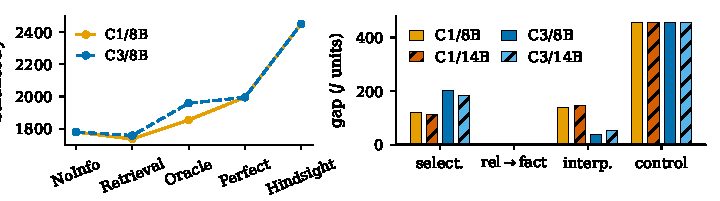
\includegraphics[width=\textwidth]{figures/fig3_ladder_c1c3}
\caption{Oracle ladder (balanced $J$, $k=3$, rerank arm): C1/8B vs C3/8B
trajectories (left; Retrieval$\to$Oracle is the selection step)
and the four gaps across all four LLM strata (right).}
\label{fig:ladder}
\end{figure}

The ladder (Table~\ref{tab:gaps}, Figure~\ref{fig:ladder}) attributes the
loss rung by rung:
\textsc{NoInfo}, \textsc{ActualRetrieval}, \textsc{OracleRelevant},
\textsc{OracleFactual}, \textsc{PerfectBelief}, \textsc{HindsightOracle} ---
separating selection, veracity, interpretation and control: the selection
gap runs $+79.5$ to $+200.7$ across arms; the oracle-relevant and
oracle-factual rungs coincide at $0.00$ in every arm (both oracle sets
saturate identically); the interpretation gap
shrinks $140.5 \to 36.4$ from naive to provenance-aware consumption; the
control gap ($+456.8$) dominates, over three times the largest LLM
interpretation gap. Exploratory regime slices concentrate the
mechanism in delay worlds.

\paragraph{Interventions on oracle evidence.}
Seven prespecified perturbations of the oracle-factual base stay positive
throughout (duplicate-top/C3 $+185$ balanced / $+215$ empirical; all
Holm-robust). Contra-injection splits
the consumers (C1 $+29$n.s.\ vs C3 $+165^*$) --- provenance-awareness pays
only where evidence starts near-perfect. Omission-intervention studies in
agentic search reach the consonant finding that static and causal utility
are near-independent~\cite{mukhopadhyay2026bridge}; our interventions fix
the policy and the environment instead of the agent's trajectory.
Counterfactual RAG methods separate causally decisive from merely
correlated evidence to build better retrievers~\cite{qin2026cfrag,liu2026cormrag},
whereas these interventions fix the downstream policy to locate where
retrieval value is lost.

\paragraph{Removal effects are consumer-conditioned and replicate.}
Leave-one-out removal of individual reranked passages moves realised
return in opposite directions across consumers: the test document removal
effect is positive for the rule consumer (C0 drop2 $+22.6$) and for
C1/14B (drop1 $+21.9$, Holm-robust). Their CIs are
$[+11.4,+33.8]$ and $[+10.4,+34.1]$; it is negative for C1/8B
(drop2 $-13.0$ $[-27.8,+0.3]$), and null for C3/8B (all CIs cross zero).
The dev-selected cells replicate on held-out queries in direction and
order (dev $+37.7$/$-16.4$ $\to$ test $+21.9$/$-13.0$), with within-query
consumer permutation rejecting chance (drop1 $p=0.0002$).
Passage value is therefore a property of the passage-consumer pairing,
measured on frozen episodes, not of the passage alone
(Figure~\ref{fig:passage}).

\begin{figure}[!tb]
\centering
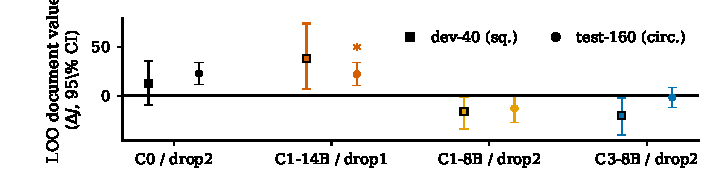
\includegraphics[width=\textwidth]{figures/fig4_passage_replication}
\caption{Leave-one-out document value by stratum (square dev-40,
circle test-160; drop1/drop2 = removed rank position;
$*$ marks the sole Holm-robust test cell, C1/14B/drop1).}
\label{fig:passage}
\end{figure}

\paragraph{Prospective passage-value prediction fails.}
A pre-specified label-free predictor of passage value (gradient-boosted
heads on deployable features; cluster-disjoint conformal calibration at
$\alpha=0.1$ over 3000 historical leave-one-out labels) does not transfer
to held-out data: rank association is marginal (pooled Spearman
$[0.079,0.168]$, C1 strata null-to-negative), coverage is $0.672$
against $[0.85,0.95]$, and out-of-fold gating is null ($[-5.7,+4.8]$). No
fresh evidence bank was built: retrospective measurement does not imply
prospective predictability (Figure~\ref{fig:vhat}).

\begin{figure}[!tb]
\centering
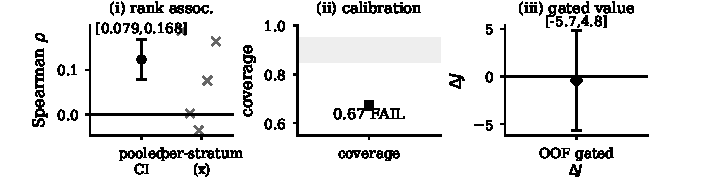
\includegraphics[width=\textwidth]{figures/fig5_vhat_failure}
\caption{Frozen predictor gate ($N=3000$ LOO labels, $\alpha=0.1$):
(i) weak positive pooled association; C1 strata null-to-negative; (ii) coverage
$0.67$ below the $[0.85,0.95]$ band;
(iii) gated value null. No bank built.}
\label{fig:vhat}
\end{figure}

\subsection{The tuned no-text comparator}
\label{sec:tuned}

We tuned a constant no-text
belief on development queries only and evaluated it
once on test: always anticipate surge.
It reaches $J=1881.1$, $+102.1$ over the prior ($p<0.0002$; Holm
significant in all 9 tuned-vs-prior and tuned-vs-real-arm comparisons;
labeled extension, SIVR $0.474$) ---
and still every real-retriever arm sits below it; the oracle C3 arms exceed
it. The
comparator rules out a straw-man prior but is prior-dependent (lost at
$-39$ normal-heavy).

A secondary multi-echelon transfer, provided in the anonymous
supplementary artifact, corroborates no-text
robustness only
(no arm beats NoInfo), reported as
environment dependence given that transfer's own projection artifact.

\section{Boundaries and limitations}
\label{sec:limitations}

The feed is synthetic, single-SKU, and finite-regime; relevance is constructed
without human annotation and nDCG is bank-specific
(heterogeneous benchmarks~\cite{thakur2021beir} are untested). Constructed
relevance judgments were independently audited against a separately
implemented provenance-derived oracle over frozen entity, event, time, and
regime state. Agreement was high (weighted $\kappa=0.848$; exact agreement
$87.5\%$; within-one-grade agreement $95.0\%$; the full confusion matrix and
nDCG sensitivity are frozen in the v4 audit manifest).
A prespecified open-weight LLM assessor was separately calibrated against
public human-judged TREC data but failed the frozen acceptance gate
($\kappa=0.461$; exact agreement $46.5\%$; within-one agreement $84.0\%$)
and was therefore excluded before any Sem2Act judging. The 160-pair packet
was balanced by constructed grade before validation, so these agreement
figures are selection-conditioned and do not establish population-wide qrel
validity.
We use one simulator, one primary fixed controller (the base-stock extension
has mixed reruns), and two open-weight models from one family. The 160 test
queries cover 63 unique texts (effective $N\approx137$); five seeds support
balanced headlines, not regime-conditional or query-difficulty inference.
The tuned comparator is prior-dependent; harm and
oracle value point the same way under all five checked weightings.

\paragraph{A sufficient condition.}
The mechanism has a simple two-state condition: if evidence causes action 1
with probability $s$ in the good state and $r$ in the bad state, with state
prevalence $p$, good-state gain $G$, and bad-state loss $L$, its realised
return is below NoInfo whenever $psG < (1-p)rL$, even though perfect
information yields $pG\geq0$. The full proof, numerical example, and
robustness table are retained in the artifact.

\section{Conclusion}
\label{sec:conclusion}

We motivate scoring decision-bound evidence at induced actions and realised
return. In this frozen pipeline, real-retriever LLM arms are non-positive at
$k=3$, naive-use harm is Holm-robust, and oracle evidence adds up to $+179$.
The ladder shows Rel$\to$Fact $0.00$, selection $+79.5$ to $+200.7$,
interpretation $140.5\to36.4$ (8B) and $144.8\to52.9$ (14B), and a
PerfectBelief$\to$Hindsight gap of $+456.8$. Evaluate retrieval against that
loop, with a no-retrieval control and matched budget.

% The full robustness table and proof are tracked in the supplement
% artifact; the compact sufficient condition is stated above.
% Marker for an exact content-page count: ECIR allows 12 content pages
% including appendices, with unlimited reference pages.
\label{endofcontent}

\bibliographystyle{splncs04}
\bibliography{references}

\end{document}
